
\documentclass[a4paper, 12pt]{book}

% XXX: why utf8x and not utf8?
\usepackage[utf8x]{inputenc}   % omogoča uporabo slovenskih črk kodiranih v formatu UTF-8 

\usepackage[slovene,english]{babel}  % naloži, med drugim, slovenske delilne vzorce
\usepackage[pdftex]{graphicx}  % omogoča vlaganje slik različnih formatov 
\usepackage{fancyhdr}          % poskrbi, na primer, za glave strani
\usepackage{amssymb}           % dodatni simboli
\usepackage{amsmath}           % eqref, npr.
\usepackage{fixltx2e}          % textsubscript etc. (XXX: used anywhere here?)
\usepackage{color}


\renewcommand*{\familydefault}{\rmdefault}  % default font family (roman)
\renewcommand{\baselinestretch}{1.3}  % ustrezen razmik med vrsticami

%oznake strani
\renewcommand{\chaptermark}[1]%
{\markboth{\MakeUppercase{\thechapter.\ #1}}{}} \renewcommand{\sectionmark}[1]%
{\markright{\MakeUppercase{\thesection.\ #1}}} \renewcommand{\headrulewidth}{0.5pt} \renewcommand{\footrulewidth}{0pt} 
\fancyhf{}
\fancyhead[LE,RO]{\sl \thepage} \fancyhead[LO]{\sl \rightmark} \fancyhead[RE]{\sl \leftmark}

\newcommand{\BibTeX}{{\sc Bib}\TeX}

\newcommand{\autfont}{\Large}
\newcommand{\titfont}{\LARGE\bf}
\newcommand{\newterm}{\textit}

%\newcommand{\TODO}{\textcolor{red}}
\newcommand{\TODO}[1]{\textcolor{red}{TODO: #1}}

\newcommand{\clearemptydoublepage}{\newpage{\pagestyle{empty}\cleardoublepage}}
\setcounter{tocdepth}{2}	      % globina kazala

% konstrukti
\newtheorem{izrek}{Izrek}[chapter]

%\newtheorem{trditev}{Trditev}[izrek]
\newenvironment{dokaz}{\emph{Dokaz.}\ }{\hspace{\fill}{$\Box$}}



\begin{document}
\selectlanguage{slovene}
\frontmatter
\setcounter{page}{1} %
\renewcommand{\thepage}{}       % preprecimo težave s številkami strani v kazalu 


%%%%%%%%%%%%%%%%%%%%%%%%%%%%%%%%%%%%%%%%
%naslovnica
\label{naslovnica}
\thispagestyle{empty}%
\begin{center}
    {\large\sc Univerza v Ljubljani\\%
      Fakulteta za računalništvo in informatiko}%
    \vskip 10em%
    {\autfont Peter Lamut\par}%
    {\titfont \TODO{Naslov diplomskega dela} \par}%
    {\vskip 2em \textsc{DIPLOMSKO DELO NA UNIVERZITETNEM ŠTUDIJU
    RAČUNALNIŠTVA IN INFORMATIKE}\par}%
    \vfill\null%
    {\large \textsc{Mentor}: doc.\ dr. Boštjan Slivnik\par}%
    {\vskip 2em \large Ljubljana 2014 \par}%
\end{center}

% prazna stran
\clearemptydoublepage


%%%%%%%%%%%%%%%%%%%%%%%%%%%%%%%%%%%%%%%%
%copyright stran
\label{copyright_page}
\thispagestyle{empty}
\vspace*{8cm}

{\small \noindent
Rezultati diplomskega dela so intelektualna lastnina avtorja in Fakultete za ra\-ču\-nal\-niš\-tvo in informatiko Univerze v Ljubljani. 
Za objavljanje ali izkoriščanje rezultatov di\-plom\-ske\-ga dela je potrebno pisno soglasje avtorja, Fakultete za ra\-ču\-nal\-niš\-tvo in 
informatiko ter mentorja.}%
\footnote{V dogovoru z mentorjem lahko kandidat diplomsko delo s pripadajočo izvorno kodo izda tudi pod katero izmed alternativnih licenc, ki ponuja določen del pravic vsem: npr. Creative Commons, GNU GPL. V tem primeru na to mesto vstavite opis licence, na primer tekst \cite{licence}

 \TODO{Morda pa res raje izdaj pod katero izmed prostih licenc?}
}


\begin{center} 
\mbox{}\vfill
% TODO: a je to potrebno tukaj? kje drugje morda?
\emph{Besedilo je oblikovano z urejevalnikom besedil \LaTeX.} 
\end{center}


% prazna stran
\clearemptydoublepage


%%%%%%%%%%%%%%%%%%%%%%%%%%%%%%%%%%%%%%%%
% stran 3 med uvodnimi listi
\noindent
\TODO{Namesto te strani {\bf vstavite} original izdane teme diplomskega 
dela s podpisom mentorja in dekana ter žigom fakultete, ki ga diplomant
dvigne v študent\-skem referatu,  preden odda izdelek v vezavo!
Glej tudi sam konec Poglavja~\ref{ch2} na strani~\pageref{pp}.}

% prazna stran
\clearemptydoublepage


%%%%%%%%%%%%%%%%%%%%%%%%%%%%%%%%%%%%%%%%
% izjava o avtorstvu
\label{izjava_avtorstvo}

\vspace*{1cm}
\begin{center} 
{\Large \textbf{\sc Izjava o avtorstvu diplomskega dela}}
\end{center}

\vspace{1cm}
\noindent Spodaj podpisani Peter Lamut,
z vpisno številko \textbf{63000200}, sem avtor diplomskega dela z naslovom:
   
\vspace{0.5cm}
\emph{\TODO{naslov diplomskega dela}}

\vspace{1.5cm}
\noindent S svojim podpisom zagotavljam, da:

\begin{itemize}
	\item sem diplomsko delo izdelal samostojno pod mentorstvom 
		doc.\ dr.\ Boštjana Slivnika,

	\item so elektronska oblika diplomskega dela, naslov (slov., angl.), povzetek (slov., angl.) ter ključne besede (slov., angl.) identični s tiskano obliko diplomskega dela,
	
	\item soglašam z javno objavo elektronske oblike diplomskega dela v zbirki ``Dela FRI''.
\end{itemize}

\vspace{1cm}

\noindent V Ljubljani, dne \TODO{datum, npr. 1. aprila 2014} \hfill Podpis avtorja:

% prazna stran
\clearemptydoublepage


%%%%%%%%%%%%%%%%%%%%%%%%%%%%%%%%%%%%%%%%
% zahvala

\label{zahvala}
\thispagestyle{empty}\mbox{}\vfill\null\it%
\TODO{Na tem mestu zapišite, komu se zahvaljujete za izdelavo diplomske naloge. Pazite, da ne boste koga pozabili. Utegnil vam bo zameriti. Temu se da izogniti tako, da pozabite na celo zahvalo.}
\rm\normalfont

% prazna stran
\clearemptydoublepage


%%%%%%%%%%%%%%%%%%%%%%%%%%%%%%%%%%%%%%%%
% kazalo
\label{kazalo}
\def\thepage{}% preprecimo tezave s stevilkami strani v kazalu 
\tableofcontents{}


% prazna stran
\clearemptydoublepage


%%%%%%%%%%%%%%%%%%%%%%%%%%%%%%%%%%%%%%%%
% povzetek
% TODO: napiši na koncu
\addcontentsline{toc}{chapter}{Povzetek}
\chapter*{Povzetek}

\TODO{Ključne besede:}%

\TODO{V vzorcu je predstavljen postopek priprave diplomskega dela z uporabo okolja \LaTeX. Vaš povzetek mora sicer vsebovati približno 100 besed, ta tukaj je odločno prekratek.}
% prazna stran
\clearemptydoublepage


%%%%%%%%%%%%%%%%%%%%%%%%%%%%%%%%%%%%%%%%
% abstract
\selectlanguage{english}
\addcontentsline{toc}{chapter}{Abstract}
\chapter*{Abstract}

\TODO{Keywords:}

\TODO{This sample document presents an approach to typesetting your BSc thesis using \LaTeX. A proper abstract should contain around 100 words which makes this one way too short.}

\selectlanguage{slovene}

% prazna stran
\clearemptydoublepage


%%%%%%%%%%%%%%%%%%%%%%%%%%%%%%%%%%%%%%%%
\mainmatter
\setcounter{page}{1}
\pagestyle{fancy}

\chapter{Uvod}

\section{Splošno o podatkovnih omrežjih}

\TODO{slovenski términ za datagrid pravilen?}

Podatkovno omrežje (angl. \textit{datagrid}) je množica med seboj
povezanih računalnikov na različnih geografskih lokacijah, ki uporabnikom
omogočajo nalaganje, hranjenje in medsebojno izmenjavanje datotek.
(TODO: vir definicije / ustrezno prilagodi definicijo)

Omeni, da imaš različne topologije, da je cilj robustnost, redundanca,
itd., sklicuj se pač na vire - odstavek ali dva max. (1 stran)

\TODO{Pa morda še kakšna slika kot primer (nariši npr. z LaTeXom - kar tako,
 za vajo)}

\section{Replikacija podatkov v podatkovnih omrežjih}

Ko uporabnik podatkovnega omrežja pošlje zahtevek za prejem neke datoteke
ali skupine datotek, se lahko pri prenašanju podatkov od strežnika do
odjemalca porabi veliko pasovne širine. Poleg tega je lahko tudi čas,
potreben za prenos, dolg. Zaradi tega je morda smiselno za posamezno
datoteko ustvariti več njenih kopij na različnih lokacijah v omrežju.
Tovrstne kopije datotek imenujemo \newterm{replike}.

Cilj ustvarjanja replik je zmanjšati porabo pasovne širine in izboljšati
odzivne čase podatkovnega omrežja (\TODO{vir, kjer sta omenjena ta dva
cilja}). Če je neka replika na voljo tudi lokalno (bliže
uporabniku, ki jo zahteva), je namreč ni potrebno vsakič znova prenašati s
strežnika, temveč se preprosto uporabi lokalna kopija.

Posamezna vozlišča (računalniki) v omrežju praviloma nimajo dovolj prostora,
da bi hranila vse replike naenkrat. Zaradi te omejitve je potrebna
strategija, na podlagi katere se odločimo, katere replike bomo hranili
na katerih vozliščih --- seveda tako, da bo zadani cilj (\TODO{številčna
referenca prej opisanega cilja?}) čim bolje izpolnjen.

Replikacijske strategije ločimo v dve skupini, in sicer poznamo
\newterm{statično replikacijo} in \newterm{dinamično replikacijo}
(\TODO{viri, kjer je to navedeno}).

\subsection{Statična replikacija}

Pri statični replikaciji za vsako posamezno vozlišče že vnaprej določimo,
katere replike bodo shranjene na njem. Problem, kako replike čim bolje
razporediti po omrežju, lahko obravnavamo kot statičen optimizacijski
problem. Zanj se sicer izkaže, da je tako NP-težek kot tudi
neaproksimativen.

\TODO{referenca kakšnega članka, ki o tem govori, npr. Čibej}

\subsection{Dinamična replikacija}

Pri dinamični replikaciji se vsako vozlišče avtonomno odloča, katere
replike bo hranilo, pri čemer se lahko množica shranjenih replik na
posameznem vozlišču skozi čas spreminja. Če vozlišče na podlagi neke
metrike oceni, da je pravkar zahtevana replika zanj bolj pomembna od ene
ali več obstoječih shranjenih replik, lahko slednje izbriše in namesto
njih shrani novo repliko.

Dinamična replikacija je boljša od statične, saj se lahko avtomatično
prilagaja morebitnim spremembam v vzorcih uporabe podatkovnega omrežja
\TODO{citat Čibej}. Poznamo veliko različnih dinamičnih replikacijskih
strategij, pri čemer je ena izmed najbolj učinkovitih algoritem
\newterm{Fast Spread} (\TODO{vir -- Ranganathan and Foster, 2001b?}).

\TODO{Fast spread prevedemo v slovenščino? "algoritem hitrega širjenja"?}


\section{Algoritem Fast Spread}
\TODO{kako deluje, kaj je ideja in problem - kako se odločiti, katere replike
zamenjati, kadar ni dovolj prostora}

tipično vozlišča nimajo prostora za vse

\subsection{LRU}
Ena varianta Fast Spreada, pri katerem zamenjamo replike, ki najdlje niso
bile uporabljene (zahtevane)

\subsection{LFU}
Različica Fast Spreada, kjer zamenjamo replike, ki so bile najmanj pogosto
uporabljane/zahtevane

\section{Trditev v člankih: izboljšava}
\TODO{2-3 odstavke. Oba članka trdita, da sta Fast Spread izboljšala glede
na LRU in LFU strategiji in dosegla boljše rezultate, ker naj bi imela boljšo
metriko za ocenjevanje vrednosti replik na nivoju posameznega vozlišča.}

Sumljivo je to, da sta članka zelo podobna, enaki odstavki, enaka slika,
skratka sum, da gre za avtoplagiatorstvo (vstavi slike, dele besedila itd.)

Motivacija: implementirati opisano ter primerjati rezultate, še posebej pa
strategiji 2011 in 2012 med seboj (ker tega v članku ni bilo) - da vidimo:\\
a) ali s strategijama dobimo opisane rezultate\\
b) neposredno primerjati obe strategiji med seboj. Članka sta si namreč
zelo podobna, neposredne medsebojne primerjave v članku 2012 pa ni.\\


\chapter{Implementacija strategij iz člankov}

\section{Opis strategij}
\subsection{Enhanced Fast Spread (EFS)}
To je članek 2011 ...

\subsection{Modified Fast Spread (MFS)}
To je pa članek 2012 ...

\section{Implementacija}
Povej, kako si naredil Python simulacijo, event SendReplica, ReceiveReplica,
vsak node je neodvisen, kako na začetku poženeš Dijsktro ...

\section{Meritve}
\subsection{Priprava simulacije}
Povej, da imaš štiri strategije (EFS, MFS, LRU, LFU). Pa povej tri scenarije,
z različnim MWG probability. V posameznem scenariju poženemo vsako izmed
štirih opisanih strategij in jih med seboj primerjamo, skupaj 12 poganjanj
(3 scenariji X 4 sstrategije)

Potem na kncu še povej, kakšni so parametri (koliko vozlišč itd. ... neka
tabela). V vsaki rundi seveda enako, razlikuje se le scenarij in pa
uporabljena trategija.

\subsection{Rezultati simulacij}

\TODO{}

Na koncu povej, da rezultatov iz člankov ni bilo možno ponoviti, zato potem
obstaja sum, da niso nič pametnega naredili, več o tem v nadaljevanju.

\chapter{Kritična presoja člankov}

\TODO{tu pa zdaj cel kup stvari}

\begin{itemize}
\item copy-paste (kako so si podobni ... tega zato zgoraj v uvodu ne pišeš, tam
le omeniš "sum plagiatorstva", tu pa potem razdelaš)

\item meritve se ne ujemajo
Povej, zakaj ... kje je spodnja meja ... kritiziraj metrike ...

\item problemi: nejasnosti, slaba metrika (razdelaj), nappake v algoritmih,
division by zero itd.

\end{itemize}


\chapter{Sklepne ugotovitve}
\TODO{nek zaključek (kakšni šalabajzerji da so) - morda kot zanimivost, da
so pošiljali plagiatorske članke še naprej v recenzijo?}



\chapter*{Sklicevanje na besedilne konstrukte \TODO{delete}}


\label{ch1}
Matematična ali popolna indukcija je eno prvih orodij, ki jih spoznamo za dokazovanje trditev pri matematičnih predmetih. 
\begin{izrek}
\label{iz:1}
Za vsako naravno število $n$ velja
\begin{equation}
n < 2^n.
\label{eq:1}
\end{equation}
\end{izrek}
\begin{dokaz}
Dokazovanje z indukcijo zahteva, da neenakost~\eqref{eq:1} najprej preverimo za najmanjše naravno število --- $0$. Res, ker je $0 < 1 = 2^0$, je neenačba~\eqref{eq:1} za $n=0$ izpolnjena.

Sledi indukcijski korak. S predpostavko, da je neenakost~\eqref{eq:1} veljavna pri nekem naravnem številu $n$, je potrebno pokazati, da je ista neenakost v veljavi tudi pri njegovem nasledniku --- naravnem številu $n+1$. Računajmo.
\begin{align}
n+1 &< 2^n + 1  \label{eq:2}\\
    &\le 2^n + 2^n \label{eq:3}\\
    &= 2^{n+1} \nonumber
\end{align} 
Neenakost~\eqref{eq:2} je posledica indukcijske predpostavke, neenakost~\eqref{eq:3} pa enostavno dejstvo, da je za vsako naravno število $n$ izraz $2^n$ vsaj tako velik kot 1. S tem je dokaz Izreka~\ref{iz:1} zaključen.
\end{dokaz}

Opazimo, da je \LaTeX\ številko izreka podredil številki poglavja.



\chapter*{Plovke: slike in tabele \TODO{delete}}
\label{ch2}
Slike in daljše tabele praviloma vključujemo v dokument kot plovke. Pozicija plovke v končnem izdelku ni pogojena s tekom besedila, temveč z izgledom strani. \LaTeX\ bo skušal plovko postaviti samostojno, praviloma na vrh strani, na kateri se na takšno plovko prvič sklicujemo. Pri tem pa bo na vsako stran končnega izdelka želel postaviti tudi sorazmerno velik del besedila. V skrajnem primeru, če imamo res preveč plovk, se bo odločil za stran popolnoma zapolnjeno s plovkami.

\section*{Formati slik}
Bitne slike, vektorske slike, kakršnekoli slike, z \LaTeX{}om lahko vključimo vse. 
Slika~\ref{pic1} je v {\tt .pdf} formatu.
\begin{figure}
\begin{center}
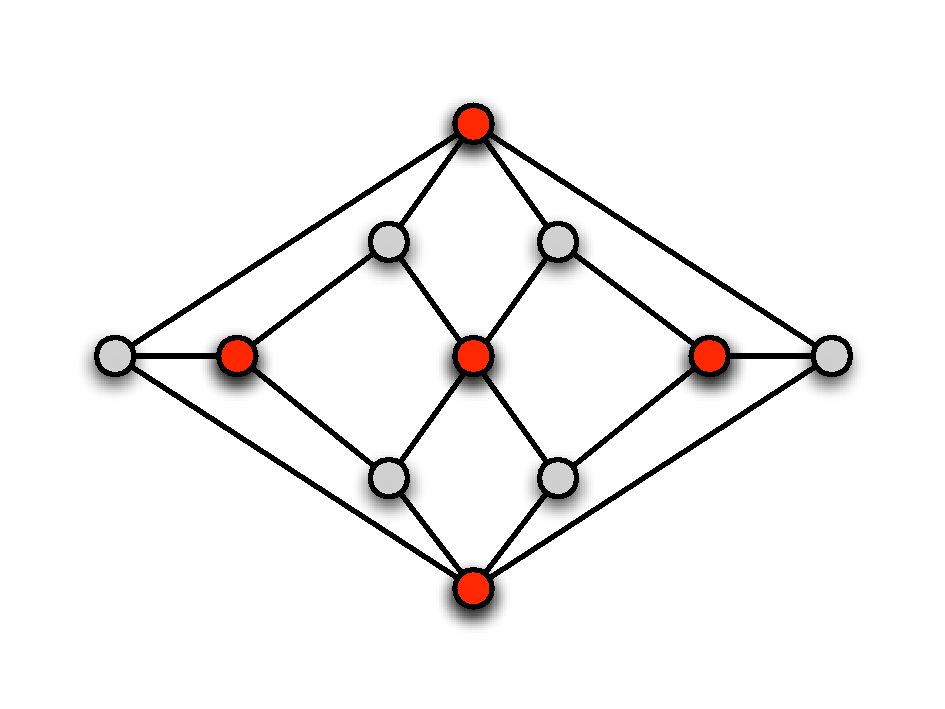
\includegraphics[width=10cm]{pic1.pdf}
\end{center}
\caption{Herschelov graf, vektorska grafika.}
\label{pic1}
\end{figure}
Pa res lahko vključimo slike katerihkoli formatov? Žal ne. Programski paket \LaTeX\ lahko uporabljamo v več dialektih. Ukaz {\tt latex} ne mara vključenih slik v formatu Portable Document Format {\tt .pdf}, ukaz {\tt pdflatex} pa ne prebavi slik v Encapsulated Postscript Formatu {\tt .eps}. 
Strnjeno v Tabeli~\ref{tbl:1}.

\begin{table}
\begin{center}
\begin{tabular}{l|ccc}
ukaz/format & {\tt .pdf} & {\tt .eps} & ostali formati \\ \hline
{\tt pdflatex} & da & ne & da \\
{\tt latex}   & ne & da  & da
\end{tabular}
\end{center}
\caption{}
\label{tbl:1}
\end{table}

Nasvet? Odločite se za uporabo ukaza {\tt pdflatex}. Vaš izdelek bo brez vmesnih stopenj na voljo v {.pdf} formatu in ga lahko odnesete v vsako tiskarno. Če morate na vsak način vključiti sliko, ki jo imate v {\tt .eps} formatu, jo vnaprej pretvorite v alternativni format, denimo {\tt .pdf}.

Včasih se da v okolju za uporabo programskega paketa \LaTeX\ nastaviti na kakšen način bomo prebavljali vhodne dokumente. Spustni meni na Sliki~\ref{pic2} odkriva uporabo \LaTeX{}a v njegovi pdf inkarnaciji --- {\tt pdflatex}.
\begin{figure}
\begin{center}

\includegraphics[width=10cm]{pic2.png}
\end{center}
\caption{Kateri dialekt uporabljati?}
\label{pic2}
\end{figure} 

Vključena Slika~\ref{pic2} je seveda bitna.

Kaj pa stran iz študentskega referata?\label{pp}
Tudi njo lahko vključimo v dokument. Toda ne kot plovko.
 



\begin{thebibliography}{99}
\label{bibliografija}

\bibitem{lf} L.\ Fortnow, ``Viewpoint: Time for computer science to grow up'',
{\it Communications of the ACM}, št.\ 52, zv.\ 8, str.\ 33--35, 2009.
\bibitem{dk1} D.\ E.\ Knuth, P. Bendix. ``Simple word problems in universal algebras'', v zborniku: Computational Problems in Abstract Algebra (ur. J. Leech), 1970, str. 263--297.
\bibitem{lat} L.\ Lamport. {\it LaTEX: A Document Preparation System}. Addison-Wesley, 1986.
\bibitem{bib} O.\ Patashnik (1998) \BibTeX{}ing. 
Dostopno na:\\ http://ftp.univie.ac.at/packages/tex/biblio/bibtex/contrib/doc/btxdoc.pdf
\bibitem{licence} licence-cc.pdf. Dostopno na: 

\end{thebibliography}


\end{document}

